\section{System Model}
%----------------------------------------------------------------------------------------%
\subsection{Network Model}
We denote as $\apSet \define \set{1,\dots,K}$ and $\mathcal{M} \define \set{1,\dots,M}$ Access Points (AP) and Edge Servers (ES) respectively in our system, as depicted in Fig. \ref{fig:system}.
We assume that both AP and ES side function at the same time slot scale which lasts for $\tau$ second ($\tau < 1$) for convenience.

\begin{figure}[ht]
    \centering
    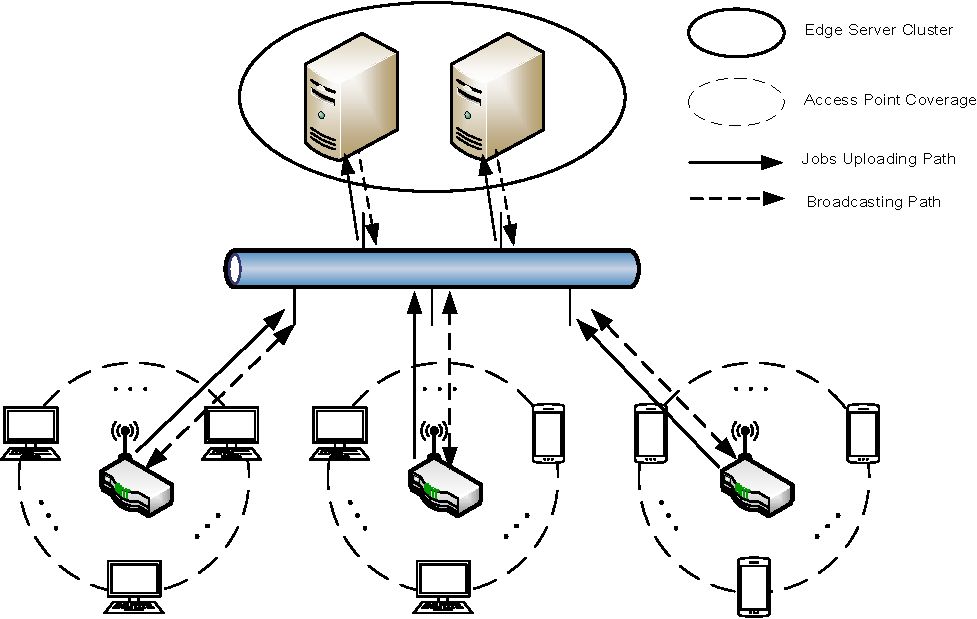
\includegraphics[width=0.45\textwidth]{system-model.pdf}
    \caption{The Illustration of MEC System Model}
    \label{fig:system}
\end{figure}


%NOTE: [job space support and arrival process]
The User Equipment (UE) is connected to the AP and offload the computation jobs on demand to the AP.
A list of types of jobs are supported on edge servers based on Virtual Machine (VM) resources, which is denoted as $\jSpace \define \set{1,\dots, J}$.
% which is obtained by statistics and denoted as $p_j \define \Pr\{\text{"j-type arrival"}\}$, where $\sum_{j\in\jSpace} p_j=1$.
Thus the job arrival process on $k$-th AP ($\forall k\in\apSet$) is compounded of the job arrivals from all UE connected, which follows the assumption as follows.
\begin{assumption}[Job Arrival Process for AP]
    The $j$-type job arrival distribution from $k$-th AP in one slot is denoted as $A_{k,j}$, which is independent and identically distributed (i.i.d) over each time slot following Bernoulli distribution as $\Bernoulli(\lambda_{k,j})$ ($\lambda_{k,j} > 0$).
    Thus average arrival rate of $j$-type jobs on $k$-th AP is $\mathbb{E}[A_{k,j}]=\lambda_{k,j}$.
\end{assumption}


%NOTE: [uploading process]
The AP itself is assumed with no computation capability, and thus the jobs are further dispatched to the edge servers for processing.
The jobs on AP will be immediately dispatched to edge servers once arrives.
The corresponding uploading delay is \emph{un-predictable} over one AP-ES link.
We assume that for $j$-type of job, the corresponding delay follows some distribution over one link from $k$-th AP to $m$-th ES ($\forall j\in\jSpace, k\in\apSet, \forall m\in\esSet$).
Without loss of generality, we assume $U_{k,m,j} \sim \Pr\{U_{k,m,j}\}$ in interval $[0, \Xi]$ where $\Xi$ is integer times of $T$.


%NOTE: [processing process] 
% VM support $\to$ independent queue $\to$ queue length $\to$ processing time
After being uploaded to edge servers, the jobs will join computation queue within the existing VM.
The different types of jobs are executed simultaneously backed by $J$ VMs on one edge server.
One VM is considered as a queue which adopt fair scheduling as First-Come-First-Serve (FCFS), while has no resource contention with other queue.
The maximum queue length is set to discourage too many jobs pending on edge servers and is denoted as $L_Q$. The job submission over the limit will be rejected and announce the AP where the job is from.

For job processing on edge servers, we adopt \emph{unrelated machines} assumption in \cite{tan-online}, where the job processing time on different servers are machine dependent and variant of resource or VM (virtual machine) constraints.
Furthermore, we denote as $C_{m,j}$ the processing time for $j$-type job on $m$-th edge serer which follows some distribution ranged from $0$ to $c$.
The processing time for one job is determined when it's about to be processed, because the computation resource for VM is allocated at that time according to the embedded resource scheduling logic.
% [abandon for \emph{unrelated machines model}]
% For convenience, we assign jobs with \emph{infinity} processing time when there are no  have no VM resource available with , and this kind of dispatching possibility will be rejected at the AP side.

%FIXME: add the following description, logically
% After the jobs being processed on ES, we consider the life cycle of that job is ended.
% The time from one job being offloaded to AP until leaving ES is denoted as the Job Completion Time (JCT), which characterize the response time in system.
%----------------------------------------------------------------------------------------%

\subsection{Information-Sharing Broadcast Model}
In the decentralized system, a information sharing scheme is indispensable to guarantee a global-wise optimal policy than local greedy policy.
However, frequent information exchange would always introduce heavy network burden and communication latency is also a severe issue which causes stale information collection. So, an efficient scheme is needed to alleviate the communication burden and aware of the stale information impact.
In this article, the proposed sharing scheme leverage a common periodic broadcast which lasting for adjustable period $T \define N \times \tau$. More specifically, the broadcasting is applied in a loose synchronized way that all the nodes (including AP and ES) starts broadcasting at the same start and is received in that period due to the stochastic latency. We further adopt the following time denotation.
\begin{align}
    t_{i,n} = i \cdot T + n \cdot \tau, (i,n=0,1,2,\dots),
\end{align}
where $t_{i,n}$ denotes the $n$-th time slot in $i$-th interval w.r.t the start point. Especially, we denote as $t_{i} \define t_{i,0}$ as the start point of each broadcasting interval, which is called \emph{broadcast point}.
And the broadcast information is a sampling of the system status, for $i$-th \emph{broadcast point}, the composed broadcast information from all the AP and ES nodes is listed as follows.
\begin{itemize}
    \item Denote as
    $\mathcal{R}(t_{i}) \define \set{ \vec{r}^{(k)}_{m,j}(t_i)|\forall k\in\apSet, m\in\esSet, j\in\jSpace }$
    the information AP cluster contains at $i$-th broadcast interval, where
    $\vec{r}^{(k)}_{m,j}(t_i) \triangleq \{ r^{(k)}_{m,j,\xi}(t_i)|\forall \xi=0,\dots,\Xi \}$
    denotes a series of counters recording the uploading time from $0$ to $\Xi$ of the $j$-type job from $k$-th AP to $m$-th ES.
    \hl{(explicit expression)}
    For each $k$-th AP ($\forall k\in\apSet$), it maintains its own information $\set{ \vec{r}^{(k)}_{m,j} | \forall m\in\esSet, j\in\jSpace}$;
    \item Denote as
    $\mathcal{Q}(t_{i}) \triangleq \set{ Q_{m,j}(t_i)|\forall m\in\esSet,j\in\jSpace }$
    the information ES cluster contains at $i$-th broadcast interval, where
    $Q_{m,j}(t_i) \triangleq (l_{m,j}(t_i), \eta_{m,j}(t_i))$
    denotes the $j$-type jobs FIFO queue on $m$-th ES, with $l_{m,j}(t_i)$ denoting the queue length and $\eta_{m,j}(t_i)$ denoting the remaining time of the job in processing.
    The $m$-th ES ($\forall m\in\esSet$) maintains information $\set{ Q_{m,j}(t_i)|\forall j\in\jSpace }$.
\end{itemize}
Thus the composed broadcasting information at $t_i$ is denoted as:
\begin{align}
    \Obsv(t_i) \define
        \Brace{
            \mathcal{R}(t_i),
            \mathcal{Q}(t_i)
        }.
\end{align}
And we notice that though $\mathcal{R}(t_{i,n})$ and $\mathcal{Q}(t_{i,n})$ also exists in each time slot, the observed information is only available at the start of each interval via broadcast. Thus the shared information is actually a uniform sampling of the whole process.

As the broadcasting latency is random due to underlaid network, different AP nodes would receive partial broadcast information at different time slots in that interval.
As the partial information updated together with stale information could not depict the status of the whole system, we only consider the time when one AP could receive the full broadcast information from ESs and other APs, which is called \emph{update latency}.
We denote as $D_{k}(t_i)$ the time \emph{update latency} for $k$-th AP ($\forall k\in\apSet$) in $i$-th interval, and $k$-th AP receives the last partial information at $t_{i} + D_{k}(t_i)$.
Due to the un-predictability of \emph{update latency}, the latency $D_{k}(t_i)$ for that AP in that interval could not share to other nodes, which implies the explicit sharing about timing information is not impossible in the distributed system.
Moreover, we assume that the broadcast interval is set as a value that always larger than the corresponding \emph{update latency}, i.e. $T > \hat{D}_k$ ($\forall k\in\apSet$), where $\hat{D}_k$ is the upper bound for $D_k$.
% [abandon, definition for update latency]
% We denote as $D^{(p)}_{k,k'}(t_i)$ the broadcast delay between $k'$-th AP and $k$-th AP ($\forall k,k'\in\apSet$), and $D^{(s)}_{k,m}(t_i)$ the broadcast delay between $m$-th ES and $k$-th AP ($\forall k\in\apSet,\forall m\in\esSet$).
% Then we denote the latency for $k$-th AP receives broadcast information from other nodes (including all ES nodes and other AP nodes) as \emph{Maximum Broadcast Latency}.
% \begin{definition}[Maximum Broadcast Latency]
%     The maximum broadcast latency is the time when AP receives whole broadcast information with respect to the broadcast point. For $k$-th AP ($\forall k\in\apSet$) the latency for $i$-th interval is given as follows.
%     \begin{align}
%         &D_{k}(t_i) \define \max\Paren{ \set{D^{(p)}_{k,k'}(t_i), D^{(s)}_{k,m}(t_i) |\forall k',k \in\apSet, \forall m\in\esSet} }
%     \end{align}
% \end{definition}

Due to the introduced periodic broadcasting design and the information receiving latency, this kind of system is inherent of the structure that decisions are always made with obsolete and partial information.
This implies that: if any agents change its decision with respect to newly-arrival broadcast information, it will disturb other agents' decisions from cooperation due to different information of system states.
Thus, it's unacceptable to update agents' policy only when the agents all come up with exactly same information.
        
In the problem formulation section, we will show that we could come up with better policy aware of the randomness of latency, and improve AP's policy in an iterative way.
Furthermore, with the help of algorithm design we could prove that our improved policy is with analytical performance bound under MDP framework.
%----------------------------------------------------------------------------------------%